%Author: Siddhesh Wani
%Date: December 22, 2015




\documentclass[12pt]{article}
\usepackage{tikz}
\usetikzlibrary{shapes.geometric, arrows}
\usepackage{hyperref}
\usepackage[a4paper]{geometry}
\usepackage[font=small]{caption}
\usepackage{listings}

%DO NOT EDIT start
%Define different shapes to be used in flowchart
\tikzstyle{startstop} = [rectangle, rounded corners, minimum width=3cm, minimum height=1cm,text centered, draw=black, fill=red!30]
\tikzstyle{io} = [trapezium, trapezium left angle=70, trapezium right angle=110, minimum width=3cm, minimum height=1cm, text centered, draw=black, fill=blue!30]
\tikzstyle{process} = [rectangle, minimum width=3cm, minimum height=1cm, text centered, draw=black, fill=orange!30]
\tikzstyle{decision} = [diamond, minimum width=3cm, minimum height=1cm, text centered, draw=black, fill=green!30]
\tikzstyle{arrow} = [thick,->,>=stealth]
\tikzstyle{connector} = [signal,draw=black,fill=olive!30]%,text width=1cm,text height=1.5cm,align=center]
%DO NOT EDIT end


\begin{document}



\section{User manual for Scilab2C}
\hypertarget{user_manual}
This section describes steps to be followed for using `Scilab2C'. Pre-requisites are mentioned followed by procedure to install `Scilab2C'.
\\

\subsection{Installation}
\subsubsection{Prerequisites}
There are few prerequisites or some packages must be pre installed before we can use `Scilab2C'. These are:
\begin{itemize}
  \item Scilab $>$=5.5.1.
  \item Scilab-Arduino toolbox (If using `Scilab2C' to generate code for Arduino)
  \item Arduino makefile (https://github.com/sudar/Arduino-Makefile). Install using `sudo apt-get install arduino-mk'.
  \item BCM2835 C library for RasberryPi (http://wiringpi.com/)
  \item RasberryPi tools (For cross compiling code for RasberryPi)
  
  Detailed instructions for installing these packages are in section \hyperlink{supporting_pkg}{`Installing supporting packages'}
\end{itemize}

\subsubsection{Installing Scilab2C}
Before we can use `Scilab2C' extension, we need to install latest version of Scilab2C. Follow following procedure to get latest source code from github repo.
\begin{itemize}
  \item Open terminal window. (Ctrl+Shift+T is shortcut).
  \item Change current directory to `/path/to/scilab/share/scilab/contrib'. Normally it is in `/usr/share/' if installed using system interface. Replace `/path/to/' by actual path to folder `scilab'. For example, if you have installed Scilab using system interface (`apt-get' on Ubuntu), then run following command in terminal:\\
  \texttt{cd /usr/share/scilab/share/scilab/contrib}
  \item Clone the git repo using following command:\\ 
\indent\indent\texttt{git clone https://github.com/siddhu8990/Scilab2C.git}
  \item Make sure a directory named `Scilab2C' is present in `contrib' folder.
  \item Open the Scilab.
  \item Run `builder.sce’ file present in `Scilab2C/2.3-1’ using `exec'. This generates binary files from source files.\\
  \indent\indent\texttt{exec(`/path/to/Scilab2C/2.3-1/builder.sce')}
  \item In `Home/.Scilab/scilabx.x.x' make a new file `.scilab' if it does not exist already. (You may need to enable `Show hidden files' from `View' menu to see .Scilab folder'.
  Open `.scilab’ using suitable editor. Add following line in this file:\\
  \indent\indent\texttt{exec(`/path/to/Scilab2C/2.3-1/loader.sce')}\\
This will load the `scilab2c' everytime scilab is started.

\end{itemize}
\hypertarget{supporting_pkg}{}
\subsubsection{Installing supporting packages}

Most of the supporting packages or libraries which are required are provided with the toolbox. But they were compiled using
latest source code available at release of toolbox. If you want to use latest libraries, steps to compile the same are listed 
below. You can follow these steps and replace old files with newly generated ones.
\begin{itemize}
 \item {\textbf{`scilab-arduino toolbox'}}
  Latest version of `scilab-arduino toolbox is available through `Atoms', toolbox installer module for Scilab.
 %\end{itemize}
  \hypertarget{tools}{}
  \item{\textbf{RasberryPi tools}}
    \begin{itemize}
   \item Make a folder named `RasberryPi tools' somewhere on the harddisk. 
   \item Open terminal and change directory to `RasberryPi tools'. Clone `Tools' repo using `git clone https://github.com/raspberrypi/tools.git'.
   \item Add location of toolchain to your `PATH' variable.\\ \texttt{`export PATH=\$PATH:/location/of/tools/folder/arm-bcm2708/gcc-linaro-arm-linux-gnueabihf-raspbian/bin'} 
  \end{itemize}

%    \item{\textbf{ BCM2835 C library for RasberryPi}}
%    \begin{itemize}
%    \item Before going further, make sure that you have installed `RasberryPi tool' following 
%    the instructions given above.
%    \item Download latest source code from `\url{http://www.airspayce.com/mikem/bcm2835}'.
%    \item Extract source code at some suitable location on harddrive.
%    \item Open the terminal window and change current directory to the location where 
%    source is extracted.
%    \item Execute following command \\
%    \texttt{./configure -host=arm CC=arm-linux-gnueabihf-gcc ar=arm-linux-gnueabihf-ar}
%    \item Then execute `make' to cross compile the library. Don't do `make install' as it is noramlly next step. 
%    \end{itemize}
   
   \item{\textbf{WiringPi C library for RaspberryPi}}
   \begin{itemize}
    \item Download latest source code from `\url{https://git.drogon.net/?p=wiringPi}'. Extract source files at some suitable location.
    \item Copy these source files to RaspberryPi at suitable location. Follow instructions given for installation. 
    \item \textbf{not complete}
   \end{itemize}

   \item{\textbf{ Cross compiling Lapack and Blas for RasberryPi}}
   \begin{itemize}
    \item Download latest source code for Lapack from `\url{http://www.netlib.org/lapack/}'. Extract source files at some suitable location.
    \item Open file `make.inc.example' given in Lapack folder using some editor.
    \item Edit following items as shown:
    \begin{itemize}
     \item FORTRAN = arm-linux-gnueabihf-gfortran
     \item LOADER = arm-linux-gnueabihf-gfortran
     \item CC = arm-linux-gnueabihf-gcc
     \item ARCH = arm-linux-gnueabihf-ar
     \item RANLIB = arm-linux-gnueabihf-ranlib
    \end{itemize}
    \item Since we are cross compiling for some other platform, normal way compiling 
    will not work.
    \item Open terminal window and change current directory to laplack directory.
    \item We will need to compile BLAS, CBLAS and Lapack separately and in same order.
    \item Change current directory to /path/to/lapack/BLAS/SRC and run `make'. This will generate `librefblas.a' in Lapack folder.
    \item Now change current directory to /path/to/laplack/CBLAS and run `make'. This will generate `libcblas.a' in Lapack folder.
    \item Now change current directory to /path/to/laplack/SRC and run `make'. This will generate `liblapack.a' in Lapack folder.
    Now replace the generated lib files in 'src/c/hardware/rasberrypi/libraries' in `scilab2c' source folder.
   \end{itemize}
   
   \item{\textbf{ GNU Scientific Library (GSL) for RasberryPi}}
   \begin{itemize}
   \item Before going further, make sure that you have installed `RasberryPi tool' following 
   the instructions given \hyperlink{tools}{here}.
   \item Get latest source code for GSL from \url{ftp://ftp.gnu.org/gnu/gsl/}.
   \item Extract source code at some suitable location on harddrive.
   \item Open the terminal window and change current directory to the location where 
   source is extracted.
   \item Execute following command \\
   \texttt{./configure -host=arm CC=arm-linux-gnueabihf-gcc ar=arm-linux-gnueabihf-ar --enable-static}
   \item Then execute `make libgsl.la' to cross compile the library. Don't do `make install' as it is noramlly next step.
   \item Library `libgsl.a' is created in folder `.libs'. By default this folder is hidden.
   \item Now replace the generated lib file in `src/c/hardware/rasberrypi/libraries' in `scilab2c' source folder.
   \item We need to set a environment variable `C\_INCLUDE\_PATH' so that arm compiler can find required files while compiling the code.
   For doing this, type following in the terminal:\\
   \texttt{export C\_INLUDE\_PATH="/path/to/gsl2.1/folder"}\\
   Replace /path/to/gsl2.1/folder by actual path on your machine.
   
   \end{itemize}
   
\end{itemize}

\subsection{Using Scilab2C for C code generation}
Scilab2C extension in Scilab can be used for generating C code from a Scilab script. Currently it supports four target platforms:
\begin{itemize}
 \item \textbf{Standalone C code}: General C code which can be compiled using any compiler
 \item \textbf{Arduino} : Arduino sketches can be generated using Scilab scripts written using `Scilab-Arduino toolbox' (A scilab-arduino extension is required)
 \item \textbf{AVR} : C code can be generated for using hardware peripherals of AVR microcontroller
 \item\textbf{Raspberry Pi} :  C code for using hardware peripherals of Raspberry Pi can be generated
\end{itemize}


You can follow following steps for generating C code using Scilab2c extension for required target platforms.
\subsubsection{Generating standalone C code}
 \begin{enumerate}
  \item Write the Scilab script first which is to be converted to C. Scilab code can contain single file or many files, but each file must be a Scilab function. 
  There must be one main Scilab file in case project contains many files, from which execution of code starts. All Scilab files must be in a single folder. 
  \item Before a Scilab file can be translated to a c code, some function annotations should be added manually. Function annotations gives information about no. of inputs/outputs, 
  their types etc. Refer \hyperlink{annot}{`Function annotations'} for more details.
  \begin{figure}[h]
  {
  \centering
   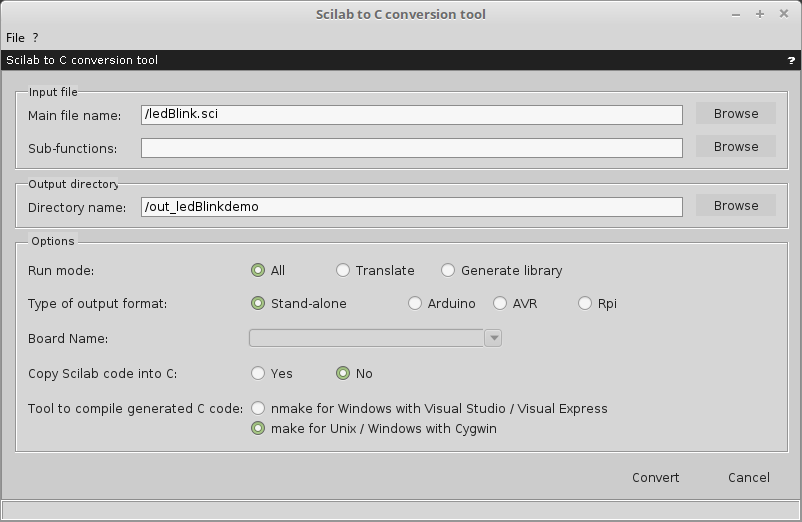
\includegraphics[scale=0.4]{img/sci2cgui}
   \caption{\small{GUI for `Scilab2C'}}
   \label{fig:gui}
  }
  \end{figure}
  
  
  \item Type `sci2c\_gui' or `scilab2c' in scilab console. This will prompt the GUI of Scilab2C toolbox as shown in figure.  \ref{fig:gui}
  
  \begin{figure}
  
  {
  \centering 
   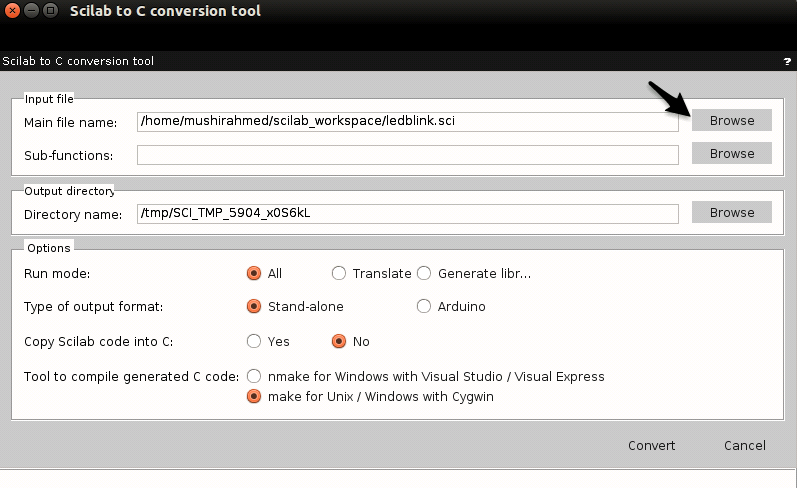
\includegraphics[scale=0.4]{img/gui_pick_file}
   \caption{\small{Select `main' scilab file for conversion}}
   \label{fig:main}
  }
  \end{figure}
  

  \item Click `Browse' next to `Main file name' textbox, browse to location of main scilab file and select it. (Refer figure \ref{fig:main})
  \item If Scilab code contains many files, select folder containing these file by clicking `Browse' next to `Sub-functions' textbox.
  \begin{figure}
  \centering
  {
   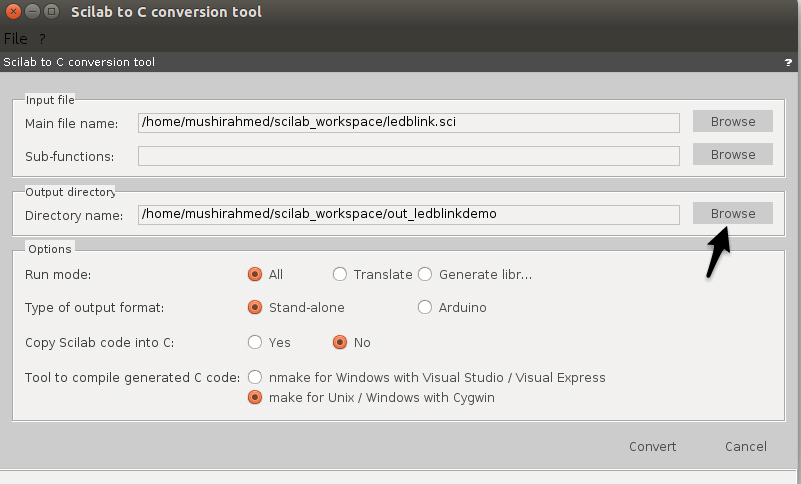
\includegraphics[scale=0.4]{img/gui_out_pickup}
   \caption {\small{Select output folder}}
   \label{fig:output}
  }
  \end{figure}

  \item Create a new folder somewhere on the disk, preferably in same folder containing Scilab files. Select this newly created folder by clicking 
  `Browse' next to `Directory name' textbox. (Refer figure \ref{fig:output}). Generated C code files are stored in this folder.
  \item Choose appropriate options from `Options' box. Different options are explained below:
  \begin{enumerate}
   \item Run mode : If only directory structure is to be generated in output directory, select `Generate library'. If only conversion of scilab files is to be done, select
   `Translate'. In case both are to be done, select `All'. 
   \item Target platform : To generate standalone C code, select `Standalone C' from dropdown. (Refer figure \ref{fig:standalone})
  \begin{figure}
  \centering
  {
   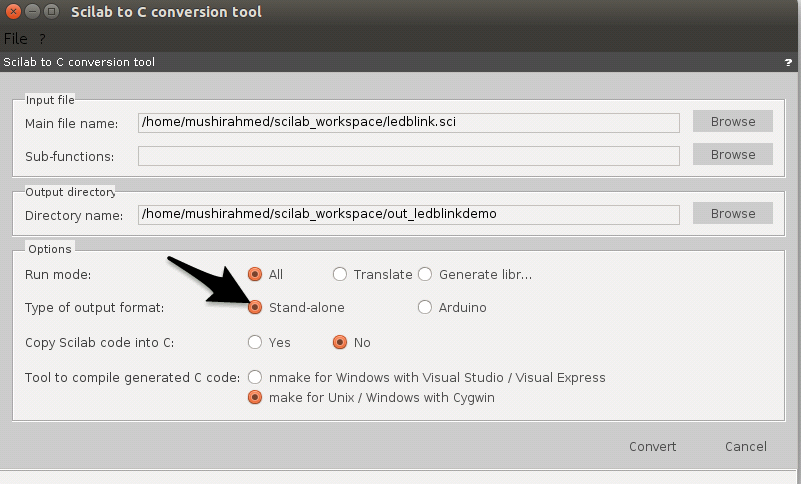
\includegraphics[scale=0.4]{img/gui_standalone}
   \caption {\small{Select `Standalone C' from dropdown}}
   \label{fig:standalone}
  }
  \end{figure}

   \item Copy Scilab code into C: Select `Yes' or `No' accordingly.
   \item Tool to compile generated C code: Select appropriate option depending upon platform on which generated code will be complied. 
  \end{enumerate}

  \item Confirm everything again and then press `Convert' button. (Refer figure \ref{fig:convert})
  \begin{figure}
  \centering
  {
   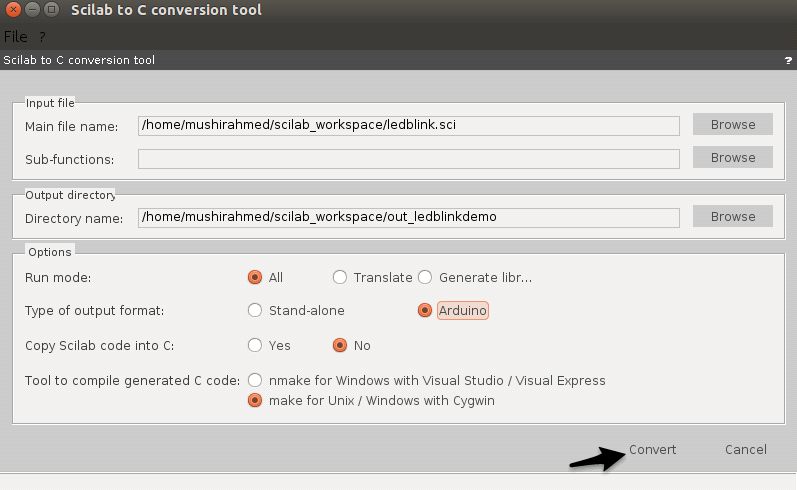
\includegraphics[scale=0.4]{img/gui_convert_btn}
   \caption {\small{Select output folder}}
   \label{fig:convert}
  }
  \end{figure}

  \item After clicking `Convert', Scilab code will be run in Scilab, to check for any errors. If code runs successfully, a prompt will occur asking if you 
  want to continue to code conversion or not. Select `Yes'. If Scilab code doesn’t run correctly then code conversion is stopped there itself. 
  Correct the Scilab code and follow the steps again.
  \item After selecting `Yes' for code conversion, code conversion starts. If code conversion is done successfully, you will see the message in command window.
  \item Generated code can be seen in output folder. By default a makefile is generated which uses `GCC' compiler to compile the C code. 
  You can compile this code using `make'. Open output folder in terminal and type `make' and press Enter. Once code is compiled successfully, it is run in terminal 
  and output can be seen in terminal window. Check the output for correctness. If code did not behave as expected, correct the Scilab code and follow the process again.

 \end{enumerate}

\subsubsection{Generating code for Arduino}
  \begin{enumerate}
  \item Write the Scilab script first which is to be converted to C. Scilab code can contain single file or many files, but each file must be a Scilab function. 
  There must be one main Scilab file in case project contains many files, from which execution of code starts. All scilab files must be in a single folder. You can verify
  working of Scilab script by runnig it on an Arduino board. Modify the script untill code behaves as expected. Once script is finalised, remove the commands 
  `open\_serial' 
  and `close\_serial'.
  
  \item Type `sci2c\_gui' or `scilab2c' in scilab console. This will prompt the GUI of Scilab2C toolbox as shown in figure  \ref{fig:gui}
  
  \item Click `Browse' next to `Main file name' textbox, browse to location of main scilab file and select it. (Refer figure \ref{fig:main})
  \item If scilab code contains many files, select folder containing these file by clicking `Browse' next to `Sub-functions' textbox.
  
  \item Create a new folder somewhere on the disk, preferably in same folder containing scilab files. Select this newly created folder by clicking 
  `Browse' next to `Directory name' textbox. (Refer figure \ref{fig:output})
  \item Choose appropriate options from `Options' box. Different options are explained below:
  \begin{enumerate}
   \item Run mode : If only directory structure is to generated in output directory, select `Generate library'. If only conversion of scilab files is to be done, select
   `Translate'. In case both are to be done, select `All'. 
   \item Target platform : To generate C code for arduino, select `Arduino' from dropdown. (Refer figure \ref{fig:arduino})
    \begin{figure}
    \centering
    {
    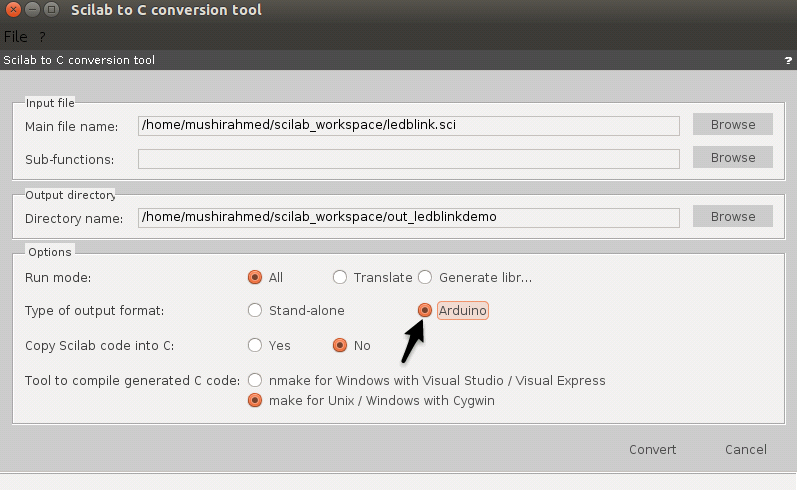
\includegraphics[scale=0.4]{img/gui_arduino}
    \caption {\small{Select `Standalone C' from dropdown}}
    \label{fig:arduino}
    }
    \end{figure}

   \item Copy scilab code into C: Select `Yes' or `No' accordingly.
   \item Tool to complie generated C code: Select appropriate option depending upon platform on which generated code will be complied. 
  \end{enumerate}
  \item Confirm everything again and then press `Convert’ button. (Refer figure \ref{fig:convert})
  \item Code conversion will start, promting different messages in command window. If conversion completes successfully, prompt will occur in command window indicationg the
  same.
  \item Generated code can be seen in output folder. A separate folder named `Arduino' is created, which contains a makefile and an arduino sketch file $-$ sci2c\_arduino.ino.
  \item Open `Makefile' using suitable text editor. Change following parameters according to board and connection:
  \begin{enumerate}
   \item  BOARD\textunderscore TAG
   \item ARDUINO\textunderscore PORT
  \end{enumerate}
  \item Open the terminal and change current directory to the directory containing modified Arduino sketch and then compile by typing `make' in terminal.
  \item If code is compiled successfully, you can upload it to arduino using `make upload' command.
  \item If code doesnot behave as expected, modify Scilab code and follow the steps again.

 \end{enumerate}
\subsubsection{Generating code for AVR}
\subsubsection{Generating code for Raspberry Pi}
\subsection{Function Annotations}
\hypertarget{annot}
Each scilab function/file should start with the function annotation section having following structure:

\begin{lstlisting}[language=scilab, frame=single]
//SCI2C: NIN=
//SCI2C: NOUT=
//SCI2C: OUT(1).TP=
//SCI2C: OUT(1).SZ(1)=
//SCI2C: OUT(1).SZ(2)=
//SCI2C: OUT(2).TP=
//SCI2C: OUT(2).SZ(1)=
//SCI2C: OUT(2).SZ(2)=
...
//SCI2C: OUT(NOUT).TP=
//SCI2C: OUT(NOUT).SZ(1)=
//SCI2C: OUT(NOUT).SZ(2)=
//SCI2C: DEFAULT_PRECISION= DOUBLE
\end{lstlisting}
Although a minimum flexibility is available in the function annotation, we suggest observing anyway the following annotation rules:
\begin{itemize}
 \item Each annotation line must start with “//SCI2C:” tag. This makes possible to hide annotations to Scilab interpreter and makes also possible to run the code without error generation.
 \item The first line of the Scilab file to be translated must start with the number of input arguments annotation “//SCI2C: NIN=”.
 \item The number of output annotations must be equal to NOUT.
 \item No blank lines should be inserted in the annotation section.
 \item The “=” symbol used in the assignment cannot be separated from the annotation specifier:
  \begin{itemize}
   \item The following annotation is correct: //SCI2C: OUT(2).TP= ...
   \item The following annotation is wrong: //SCI2C: OUT(2).TP = ...
  \end{itemize}
 \item To be sure that the annotation of the user code has been correctly interpreted by Sci2C please check 
 the .ann file generated by Sci2C when the .sci file is read. Supposing that we are translating file myfun.sci, 
 the user should access the myfun.ann file generated by Sci2C in order to check that it contains the right annotations.
\end{itemize}

Each of the above tag is explained below:
\begin{enumerate}
 \item \textbf{NIN}\\
 NIN specifies the number of input arguments that the function can handle. This tag is useful for Sci2C functions that can handle different 
 number of input arguments, whereas it is not useful for User2C functions because they must work with a fixed number of input arguments. 
 NIN annotation tag makes use of the following syntax:
 \begin{center}
  //SCI2C: NIN=    number
 \end{center}
  where:\\
   \textit{number} is a number specifying the number of input arguments.
 \item \textbf{NOUT}\\
 NOUT specifies the number of output arguments the function can handle. This tag is useful for Sci2C functions that can handle different number of output arguments, 
 whereas it is not useful for User2C functions because they must work with a fixed number of output arguments.
  NOUT annotation tag makes use of the following syntax:
 \begin{center}
  //SCI2C: NOUT=    number
 \end{center}
  where:\\
   \textit{number} is a number specifying the number of output arguments.
 \item \textbf{TP}\\
 This tag specifies the type (and precision) of the returned output arguments. The annotation section must contain a number of TP annotation tags equal 
 to the number of output arguments. TP annotation tag makes use of the following syntax:
  \begin{center}
    //SCI2C: OUT(k).TP=    type expression
  \end{center}
where:\\
  \textit{k} is a sequential number (from 1 to NOUT) indicating that we are annotating the type and precision of the k-th output argument.\\
  \textit{type expression} is an expression that specifies the type and precision of the k-th output argument. Type expression can be a 
  composition of the type annotation functions listed below. In the following list, for each type annotation
  function it is specified its number of input and output arguments, and the result returned:\\
  \begin{itemize}
   \item \textbf{FA\_TP\_S}: NInArgs = 0, NOutArgs=1; when this function is invoked it means that the output argument is of “s” type (real, float single precision).
   \item \textbf{FA\_TP\_D}: NInArgs = 0, NOutArgs=1; when this function is invoked it means that the output argument is of “d” type (real, float double precision)..
   \item \textbf{FA\_TP\_C}: NInArgs = 0, NOutArgs=1; when this function is invoked it means that the output argument is of “c” type (complex, float single precision).
   \item \textbf{FA\_TP\_Z}: NInArgs = 0, NOutArgs=1; when this function is invoked it means that the output argument is of “z” type (complex, float double precision).
   \item \textbf{FA\_TP\_UINT8}: NInArgs = 0, NOutArgs=1; when this function is invoked it means that the output argument is of “u8” type (unsigned, 8 bit precision).
   \item \textbf{FA\_TP\_UINT16}: NInArgs = 0, NOutArgs=1; when this function is invoked it means that the output argument is of “u16” type (unsigned, 16 bit precision).
   \item \textbf{FA\_TP\_INT8}: NInArgs = 0, NOutArgs=1; when this function is invoked it means that the output argument is of “i8” type (signed, 8 bit precision).
   \item \textbf{FA\_TP\_INT16}: NInArgs = 0, NOutArgs=1; when this function is invoked it means that the output argument is of “i16” type (signed, 16 bit precision).
   \item \textbf{FA\_TP\_USER}: NInArgs = 0 NOutArgs=1; when this function is invoked it means that the output argument must be specified by the user in the Scilab code. More specifically, the type and precision can be specified in the Scilab code by using the following data annotation functions: float, double, floatcomplex, doublecomplex (see section dedicated to data annotation for more details). 
   \item \textbf{IN(m).TP}: NInArgs = 0 NOutArgs=1; when this function is invoked it will return the type and precision of the m-th input argument.
  \end{itemize}

  \item \textbf{SZ}\\
  This tag specifies the size of the returned output arguments. The annotation section must contain a number of SZ annotation tags equal 
  to twice the number of output arguments, this is because for each output argument two SZ annotations are required, the first one 
  specifying the number of rows and the second one specifying the number of columns of the output argument. SZ annotation tag makes use of the following syntax:
  \begin{center}
      //SCI2C: OUT(k).SZ(1)= size expression\\
      //SCI2C: OUT(k).SZ(2)= size expression
  \end{center}
where:
  \textit{k} is a sequential number (from 1 to NOUT) indicating that we are annotating the size of the k-th output argument.
  \textit{.SZ} is assumed to be a 2-element string array indicating the number of rows (.SZ(1)) and columns (.SZ(2)) of the 
  k-th output argument. Number of rows and columns can be specified by using numbers or symbols. 
  \textit{size expression} is an expression that specifies the size of the k-th output argument. Size expression can be a 
  composition of the size annotation functions listed below. For each size annotation function 
  it is specified its number of input and output arguments, and the result returned:
  \begin{itemize}
   \item \textbf{FA\_SZ\_1}: NInArgs = 1, NOutArgs=1; this function extracts the first element of a 
   two-element string array. It is useful to extract the number of rows from the size of an input 
   argument as shows the following example:
   \begin{center}
      //SCI2C: OUT(k).SZ(2)= FA\_SZ\_1(IN(m).SZ) 
   \end{center}
  In this annotation we are indicating that the number of columns (.SZ(2)) of the k-th output argument is equal to the number 
  of rows of the m-th input argument. An equivalent annotation is the following one:
  \begin{center}
    //SCI2C: OUT(k).SZ(2)= IN(m).SZ(1)
  \end{center}

  \item \textbf{FA\_SZ\_2}: NInArgs = 1, NOutArgs=1; this function extracts the second element of a two-element string array. 
  It is useful to extract the number of columns from the size of an input argument as shows the following example:
  \begin{center}
    //SCI2C: OUT(k).SZ(1)= FA\_SZ\_2(IN(m).SZ)
  \end{center}
  In this annotation we are indicating that the number of rows (.SZ(1)) of the k-th output argument is equal to the number 
  of columns of the m-th input argument. An equivalent annotation is the following one:
  \begin{center}
    //SCI2C: OUT(k).SZ(1)= IN(m).SZ(2)
  \end{center}

  \item \textbf{FA\_SZ\_OPDOTSTAR}: NInArgs = 2, NOutArgs=1; this function accepts two input .SZ string arrays and returns a .SZ string array which specifies the size of the output argument returned by the $.*$ operator. 
  This is a useful function to annotate functions that work with two input arguments and return a single output argument whose size is a function of the sizes of the input arguments according to the 
  rules used for the $.*$ operator. For example for ``$./$'', ``$.*$'' ``$.\hat{}$'' operators the following size annotations can be adopted:
  \begin{center}
    //SCI2C: OUT(1).SZ(1)= FA\_SZ\_1(FA\_SZ\_OPDOTSTAR(IN(1).SZ,IN(2).SZ))\\
    //SCI2C: OUT(1).SZ(2)= FA\_SZ\_2(FA\_SZ\_OPDOTSTAR(IN(1).SZ,IN(2).SZ))
  \end{center}

    \item \textbf{FA\_SZ\_OPHAT}: NInArgs = 2, NOutArgs=1; this function is an alias for FA\_SZ\_OPDOTSTAR. This is because $\hat{}$ and $.*$ operators have the same behaviour for what concerns the size of the output argument.

    \item \textbf{FA\_SZ\_OPMINUS}: NInArgs = 2, NOutArgs=1; this function is an alias for FA\_SZ\_OPDOTSTAR. This is because ``$-$'' and ``$.*$'' operators have the same behaviour for what concerns the size of the output argument.
    
    \item \textbf{FA\_SZ\_OPPLUSA}: NInArgs = 2, NOutArgs=1; this function is an alias for FA\_SZ\_OPDOTSTAR. This is because ``$+$'' and ``$.*$`` operators have the same behaviour for what concerns the size of the output argument.

    \item \textbf{FA\_SZ\_OPSTAR}: NInArgs = 2, NOutArgs=1;  this function accepts two input .SZ string arrays and returns a .SZ string array which specifies the size of the output argument returned by the $*$ operator. This is a useful 
    function to annotate functions that work with two input arguments and return a single output argument whose size is a function of the sizes of the input arguments according to the rules used for the $*$ operator. 
    See the following example:
    \begin{center}
	//SCI2C: OUT(1).SZ(1)= FA\_SZ\_1(FA\_SZ\_OPSTAR(IN(1).SZ,IN(2).SZ))\\
	//SCI2C: OUT(1).SZ(2)= FA\_SZ\_2(FA\_SZ\_OPSTAR(IN(1).SZ,IN(2).SZ))
    \end{center}
    
    \item \textbf{FA\_ADD}:  NInArgs = 2, NOutArgs=1;  this function accepts two input strings returns a string which contains the sum of the two input strings according to the following rules:
    \begin{center}
	FA\_ADD('3','43') = '46'\\
	FA\_ADD('symbol1','43') = 'symbol1+43'\\
	FA\_ADD('symbol1','symbol2') = 'symbol1+symbol2'\\
    \end{center}
    As shown in the examples above FA\_ADD performs a sum of the two input strings when both strings contain numbers, otherwise the output string will be a composition of the two input strings 
    with the ''$+$`` symbol. This function is used to annotate functions that generate outputs whose size is given by adding the sizes of the input arguments.
    Let's consider, as example, the OpRc operator which implements the row concatenation (''[,]``). Row concatenation is shown in the following example:\\
A = [1 2 3; 3 4 5];\\
B = [4 5; 1 1];\\
C = [A,B]\\
According to the code above C is equal to [1 2 3 4 5; 3 4 5 1 1]  \\
In terms of size, the number of rows of C is equal to the number of rows of A (or B) and the number of columns of C is equal to the number of columns of A plus the number of columns of B. 
It follows that the right annotation for the OpRc operator is:
\begin{center}
  //SCI2C: NIN=          2
  //SCI2C: NOUT=         1
  //SCI2C: OUT(1).TP=  FA\_TP\_MAX(IN(1).TP,IN(2).TP)
  //SCI2C: OUT(1).SZ(1)= IN(1).SZ(1)
  //SCI2C: OUT(1).SZ(2)= FA\_ADD(IN(1).SZ(2),IN(2).SZ(2))
\end{center}
  
  \item \textbf{FA\_SUB}:  NInArgs = 2, NOutArgs=1;  this function has the same behaviour of FA\_ADD, but it performs a subtraction between the two input arguments.
  \item \textbf{FA\_MUL}:  NInArgs = 2, NOutArgs=1;  this function has the same behaviour of FA\_ADD, but it performs a multiplication between the two input arguments.
  \item \textbf{FA\_DIV}:  NInArgs = 2, NOutArgs=1;  this function has the same behaviour of  FA\_ADD, but it performs a division between the two input arguments.
  \item \textbf{FA\_MAX}:  NInArgs = 2, NOutArgs=1;  this function has the same behaviour of FA\_ADD, but computes the maximum between the two arguments. 
  When the two input arguments don't specify a number, the output argument will be equal to the first input argument.
  See the following examples:\\
  FA\_MAX('3','55') = '55'\\
  FA\_MAX('3','a') = '3'\\
  FA\_MAX('cccc','a') = 'cccc'\\
  FA\_MAX('cccc','88888888888888') = 'cccc'\\
  
  \item \textbf{FA\_INT}:    NInArgs = 1, NOutArgs=1;  this function truncates to int the input argument only if the input argument is a string specifying a number. 
  See the following examples:\\
FA\_INT('3.444') = '3'\\
FA\_INT('-3.444') = '-3'\\
FA\_INT('ciao') = 'ciao'\\



  \end{itemize}

  

 \end{enumerate}


\end{document}